\documentclass{standalone}
\usepackage{tikz}
\usetikzlibrary{patterns}
\usetikzlibrary{positioning}
\usetikzlibrary{patterns, positioning}
\usetikzlibrary{shapes.misc}
\usepackage[outline]{contour}
\contourlength{1.5pt} 
\usepackage[sfdefault]{ClearSans}

\begin{document}
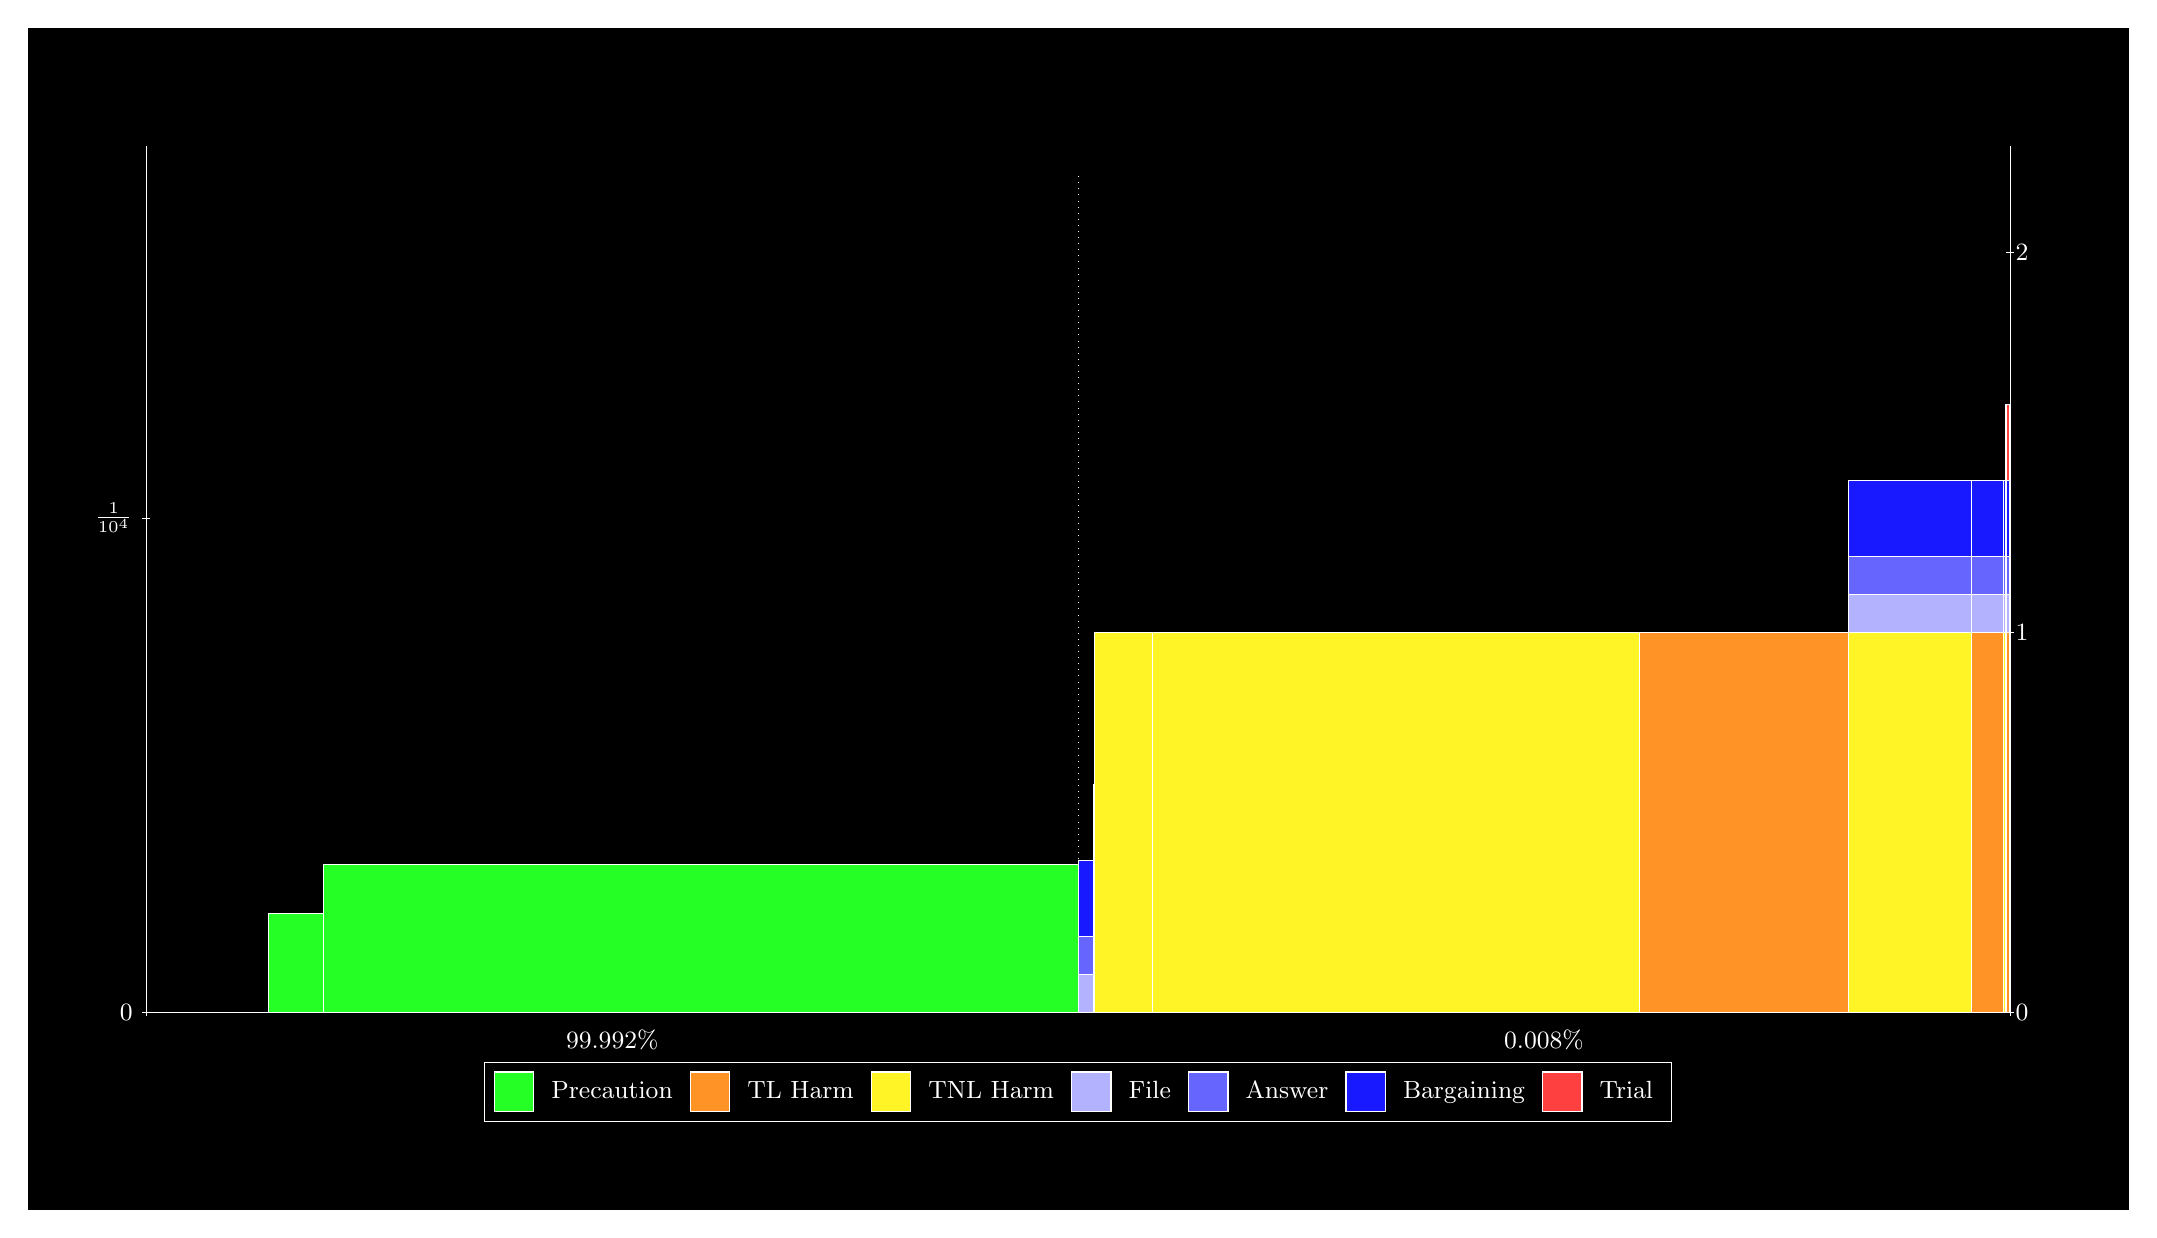
\begin{tikzpicture}
\draw[fill=black] (0,0) rectangle (26.667,15);
\draw[fill=green!85,draw=white,very thin] (3.0469,2.5) rectangle (3.7465,3.7564);
\draw[fill=green!85,draw=white,very thin] (3.7465,2.5) rectangle (13.333,4.3846);
\draw[fill=blue!30,draw=white,very thin] (13.333,2.5) rectangle (13.53,2.9827);
\draw[fill=blue!60,draw=white,very thin] (13.333,2.9827) rectangle (13.53,3.4653);
\draw[fill=blue!90,draw=white,very thin] (13.333,3.4653) rectangle (13.53,4.4307);
\draw[fill=blue!30,draw=white,very thin] (13.53,2.5) rectangle (13.535,2.9827);
\draw[fill=blue!60,draw=white,very thin] (13.53,2.9827) rectangle (13.535,3.4653);
\draw[fill=blue!90,draw=white,very thin] (13.53,3.4653) rectangle (13.535,4.4307);
\draw[fill=red!75,draw=white,very thin] (13.53,4.4307) rectangle (13.535,5.396);
\draw[fill=green!85,draw=white,very thin] (13.535,2.5) rectangle (14.279,2.5001);
\draw[fill=yellow!85,draw=white,very thin] (13.535,2.5001) rectangle (14.279,7.3268);
\draw[fill=green!85,draw=white,very thin] (14.279,2.5) rectangle (20.46,2.5001);
\draw[fill=yellow!85,draw=white,very thin] (14.279,2.5001) rectangle (20.46,7.3268);
\draw[fill=green!85,draw=white,very thin] (20.46,2.5) rectangle (23.114,2.5001);
\draw[fill=orange!85,draw=white,very thin] (20.46,2.5001) rectangle (23.114,7.3268);
\draw[fill=yellow!85,draw=white,very thin] (23.114,2.5) rectangle (24.672,7.3267);
\draw[fill=blue!30,draw=white,very thin] (23.114,7.3267) rectangle (24.672,7.8094);
\draw[fill=blue!60,draw=white,very thin] (23.114,7.8094) rectangle (24.672,8.292);
\draw[fill=blue!90,draw=white,very thin] (23.114,8.292) rectangle (24.672,9.2574);
\draw[fill=orange!85,draw=white,very thin] (24.672,2.5) rectangle (25.079,7.3267);
\draw[fill=blue!30,draw=white,very thin] (24.672,7.3267) rectangle (25.079,7.8094);
\draw[fill=blue!60,draw=white,very thin] (24.672,7.8094) rectangle (25.079,8.292);
\draw[fill=blue!90,draw=white,very thin] (24.672,8.292) rectangle (25.079,9.2574);
\draw[fill=green!85,draw=white,very thin] (25.079,2.5) rectangle (25.111,2.5001);
\draw[fill=yellow!85,draw=white,very thin] (25.079,2.5001) rectangle (25.111,7.3268);
\draw[fill=blue!30,draw=white,very thin] (25.079,7.3268) rectangle (25.111,7.8095);
\draw[fill=blue!60,draw=white,very thin] (25.079,7.8095) rectangle (25.111,8.2921);
\draw[fill=blue!90,draw=white,very thin] (25.079,8.2921) rectangle (25.111,9.2575);
\draw[fill=green!85,draw=white,very thin] (25.111,2.5) rectangle (25.113,2.5001);
\draw[fill=orange!85,draw=white,very thin] (25.111,2.5001) rectangle (25.113,7.3268);
\draw[fill=blue!30,draw=white,very thin] (25.111,7.3268) rectangle (25.113,7.8095);
\draw[fill=blue!60,draw=white,very thin] (25.111,7.8095) rectangle (25.113,8.2921);
\draw[fill=blue!90,draw=white,very thin] (25.111,8.2921) rectangle (25.113,9.2575);
\draw[fill=yellow!85,draw=white,very thin] (25.113,2.5) rectangle (25.116,7.3267);
\draw[fill=blue!30,draw=white,very thin] (25.113,7.3267) rectangle (25.116,7.8094);
\draw[fill=blue!60,draw=white,very thin] (25.113,7.8094) rectangle (25.116,8.292);
\draw[fill=blue!90,draw=white,very thin] (25.113,8.292) rectangle (25.116,9.2574);
\draw[fill=red!75,draw=white,very thin] (25.113,9.2574) rectangle (25.116,10.223);
\draw[fill=orange!85,draw=white,very thin] (25.116,2.5) rectangle (25.16,7.3267);
\draw[fill=blue!30,draw=white,very thin] (25.116,7.3267) rectangle (25.16,7.8094);
\draw[fill=blue!60,draw=white,very thin] (25.116,7.8094) rectangle (25.16,8.292);
\draw[fill=blue!90,draw=white,very thin] (25.116,8.292) rectangle (25.16,9.2574);
\draw[fill=red!75,draw=white,very thin] (25.116,9.2574) rectangle (25.16,10.223);
\draw[fill=green!85,draw=white,very thin] (25.16,2.5) rectangle (25.165,2.5001);
\draw[fill=yellow!85,draw=white,very thin] (25.16,2.5001) rectangle (25.165,7.3268);
\draw[fill=blue!30,draw=white,very thin] (25.16,7.3268) rectangle (25.165,7.8095);
\draw[fill=blue!60,draw=white,very thin] (25.16,7.8095) rectangle (25.165,8.2921);
\draw[fill=blue!90,draw=white,very thin] (25.16,8.2921) rectangle (25.165,9.2575);
\draw[fill=red!75,draw=white,very thin] (25.16,9.2575) rectangle (25.165,10.223);
\draw[fill=green!85,draw=white,very thin] (25.165,2.5) rectangle (25.167,2.5001);
\draw[fill=orange!85,draw=white,very thin] (25.165,2.5001) rectangle (25.167,7.3268);
\draw[fill=blue!30,draw=white,very thin] (25.165,7.3268) rectangle (25.167,7.8095);
\draw[fill=blue!60,draw=white,very thin] (25.165,7.8095) rectangle (25.167,8.2921);
\draw[fill=blue!90,draw=white,very thin] (25.165,8.2921) rectangle (25.167,9.2575);
\draw[fill=red!75,draw=white,very thin] (25.165,9.2575) rectangle (25.167,10.223);
\draw[white,very thin] (1.5,2.5) -- (1.5,13.5);
\draw[white,very thin] (1.45,2.5) -- (1.55,2.5);
\node[font=\small,text=white, anchor=east] at (1.45, 2.5) {0};
\draw[white,very thin] (1.45,8.7821) -- (1.55,8.7821);
\node[font=\small,text=white, anchor=east] at (1.45, 8.7821) {$\frac{1}{10^{4}}$};

\draw[white,dotted,very thin] (13.333,2.83) -- (13.333,13.17);
\draw[white,very thin] (25.167,2.5) -- (25.167,13.5);
\draw[white,very thin] (25.117,2.5) -- (25.217,2.5);
\node[font=\small,text=white, anchor=west] at (25.117, 2.5) {0};
\draw[white,very thin] (25.117,7.3267) -- (25.217,7.3267);
\node[font=\small,text=white, anchor=west] at (25.117, 7.3267) {1};
\draw[white,very thin] (25.117,12.153) -- (25.217,12.153);
\node[font=\small,text=white, anchor=west] at (25.117, 12.153) {2};

\draw[white,very thin] (1.5,2.5) -- (25.167,2.5);
\draw[white,very thin] (1.5,2.45) -- (1.5,2.55);
\node[font=\small,text=white, anchor=north] at (1.5, 2.45) {};
\draw[white,very thin] (25.167,2.45) -- (25.167,2.55);
\node[font=\small,text=white, anchor=north] at (25.167, 2.45) {};

\node[font=\small,text=white,anchor=south] at (7.4167, 1.9) {99.992\%};
\node[font=\small,text=white,anchor=south] at (19.25, 1.9) {0.008\%};
\draw (13.3333,2.5) node (B) {};
\begin{scope}[align=center]
\matrix[scale=0.5,draw=white,below=0.5cm of B,nodes={draw},column sep=0.1cm]{
\node[rectangle,draw,minimum width=0.5cm,minimum height=0.5cm,fill=green!85]{}; & \node[draw=none,font=\small,text=white]{Precaution}; &
\node[rectangle,draw,minimum width=0.5cm,minimum height=0.5cm,fill=orange!85]{}; & \node[draw=none,font=\small,text=white]{TL Harm}; &
\node[rectangle,draw,minimum width=0.5cm,minimum height=0.5cm,fill=yellow!85]{}; & \node[draw=none,font=\small,text=white]{TNL Harm}; &
\node[rectangle,draw,minimum width=0.5cm,minimum height=0.5cm,fill=blue!30]{}; & \node[draw=none,font=\small,text=white]{File}; &
\node[rectangle,draw,minimum width=0.5cm,minimum height=0.5cm,fill=blue!60]{}; & \node[draw=none,font=\small,text=white]{Answer}; &
\node[rectangle,draw,minimum width=0.5cm,minimum height=0.5cm,fill=blue!90]{}; & \node[draw=none,font=\small,text=white]{Bargaining}; &
\node[rectangle,draw,minimum width=0.5cm,minimum height=0.5cm,fill=red!75]{}; & \node[draw=none,font=\small,text=white]{Trial}; \\\\
};\end{scope}

\end{tikzpicture}
\end{document}